\begin{figure}[tbp]
\centering
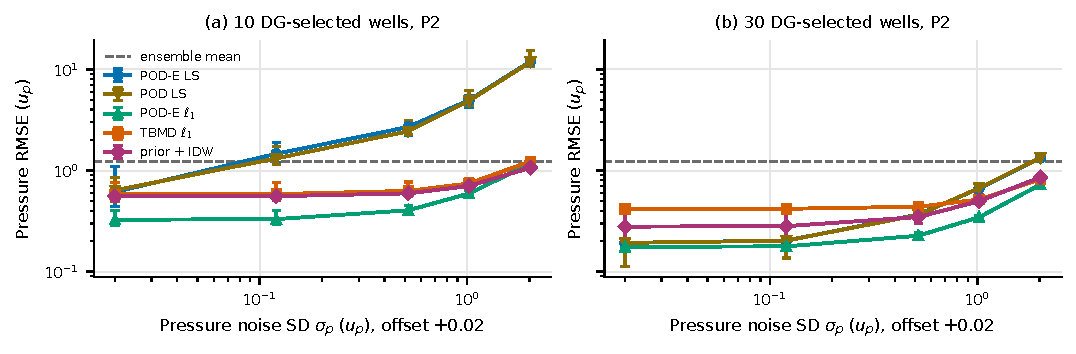
\includegraphics[width=\textwidth]{../../../../studies/brugge_sparse_sensing/figures/fig6_noise.pdf}
\caption{Effect of measurement noise in P2 for (a) 10 and (b) 30 DG-selected wells measuring pressure and $S_o$. Noise standard deviations are $(\sigma_p,\sigma_{S_o})\in\{(0,0),(0.1,0.005),(0.5,0.01),(1,0.02),(2,0.05)\}$ in ($u_p$, dimensionless); the horizontal axis shows $\sigma_p+0.02\,u_p$ so that the noise-free case appears on the logarithmic axis. Markers: median over folds of the per-fold mean over ten noise draws (one evaluation at zero noise); bars: interquartile range over folds; dashed grey: ensemble-mean prior.}
\label{fig:noise}
\end{figure}
